\section{Web 3.0 --- Das Semantische Web}
\label{sec:hauptteil}

\subsection{Auswirkungen auf die Gesellschaft}

Schon heute drehen sich die meisten der regelmäßig ausgeführtem Aktivitäten im Internet um \buzz{Informationen}\index{Information} oder gar \buzz{Wissen}\index{Wissen}, nicht um \buzz{Daten}\index{Daten}. So sind 56\% der im Digitalindex 2014 befragten Deutschen überzeugt, im Internet die automatisch die aktuellsten Informationen zu finden, 60\% sucht benötigte Informationen zuerst im Netz\footnote{vgl. \cite{d21}, Seite 6}. Die Erwartungen bzgl. Aktualität und Informationsgehalt an das \buzz{World Wide Web}\index{Web!World Wide} sind also sehr hoch. 

\begin{figure}[H]
\begin{center}
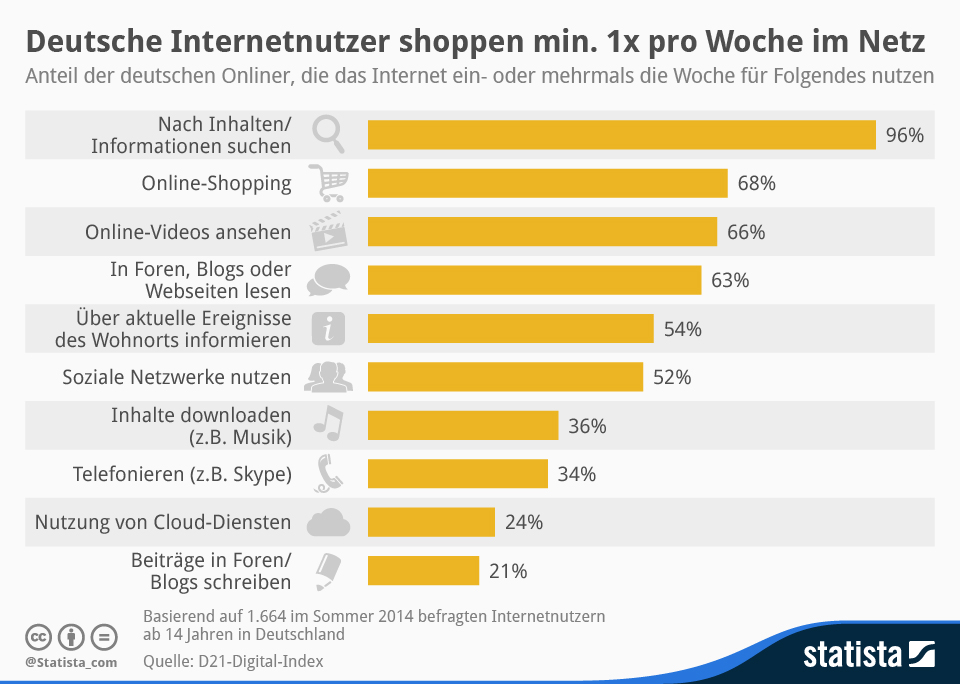
\includegraphics[width=0.67\textwidth]{inetnutzung.jpg}
\caption[Internetnutzung in Deutschland 2014]{Internetnutzung in Deutschland 2014\protect\footnotemark}
\label{pic:inetnutzung}
\end{center}
\end{figure}
\footnotetext{\cite{d21}, Seite 37}

Unter den Top 10 der regelmäßig durchgeführten Tätigkeiten der Befragten im Web finden sich die informationsorientierten Tätigkeiten „nach Inhalten/Informationen suchen“ auf Platz eins, „über aktuelle Ereignisse des Wohnorts informieren“ auf Platz 6 und die Erfassung eigener Daten auf dem 10. Platz\footnote{vgl. \cite{d21}, Seite 37}. Weitere Tätigkeiten wie „Soziale Netzwerke nutzen“ (Platz 7) bzw. „Online--Videos ansehen“ (Platz 3) sowie „Online--Shopping“ (Platz 2) nutzen Internetangebote, die per Design sehr gut mit Taxonomien, Meta--Daten und Verknüpfungen ausgestattet sind.

In den TV--Werbespots von Google und Apple werden Verbraucher gezielt auf entsprechend formulierte Anfragemöglichkeiten hingewiesen\footnote{z.B. „Ok Google, zeig mir mal den schnellsten Weg in den Münchner Tierpark?“, \cite{okg:tierpark}}. Somit werden die Möglichkeiten wie Routenplanung, Musiktitelerkennung, Wettervorhersage und andere, die schon heute durch einzelne Anwendungen zur Verfügung gestellt werden in einer Oberfläche Gebündelt und in das Bewusstsein der Verbraucher gebracht.

\label{probleme}
Neben dem offensichtlichen Nutzen des \buzz{World Wide Web}\index{Web!World Wide} bringt die Entwicklung des Webs auch negative Auswirkungen auf die Gesellschaft. 
Dies äußert sich in der Besorgnis von 60\% der Nutzer über die im Internet möglicherweise verfügbaren persönlichen Daten\footnote{vgl. \cite{d21}, Seite 6}. Bei der Nutzung von Webdiensten der öffentlichen Verwaltung haben 65\% der Befragten Angst vor Datendiebstahl, und 73\% der Deutschen haben ein starkes Interesse daran, wie Behörden mit den Daten der Bürger umgeht\footnote{vgl. \cite{d21gov}, Seite 9 bzw. Seite 34}.  Sowohl fiktive\footnote{z.B. Ozeanien in \cite{orwell}} also auch reale\footnote{z.B. die DDR, vgl. \cite{wp:stasi}} Unrechtsstaaten basieren auf der intensiven Erfassung und Auswertung von personenbezogener Daten der Bürger, was entsprechende Befürchtungen nährt und erklärt.

Man kann davon ausgehen, dass mit weiter wachsenden Datenmengen, aber auch durch entsprechenden Wachstum an generierten und erfassten Informationen und Wissen sowohl die positiven Erwartungen als auch die Befürchtungen und Ängste in der Bevölkerung zunehmen werden.

\subsection{Auswirkungen auf die Wirtschaft}

Schon heute haben Unternehmen erkannt, dass es nicht ausreicht, immer mehr Daten anzuhäufen. Der Schritt von \buzz{Big Data} zu \buzz{Big Information}\index{Big Information|textbf} bringt Benutzerfreundlichkeit und echten Mehrwert für Unternehmen\footnote{vgl. \cite{odnsbi}}. In großen Unternehmen wird unter den Schlagwort \buzz{Business Intelligence}\index{Business Intelligence} bzw. \buzz{Online Analytical Processing} mit unterschiedlichen Technologien aus den im \buzz{Data Warehouse}\index{Data Warehouse} gespeicherten Daten Informationen und informatives Wissen zu extrahieren, auf dem dann Entscheidungen und Handlungen basieren können. 

Schon in der Vergangenheit haben Fortschritte in der Daten-- und Informationsbearbeitung erhebliche Auswirkungen auf die Wirtschaft gehabt. So war die Entwicklung der Telegraphie ein wichtiger Schritt für die Meteorologie, da hiermit zeitnahe Datensammlung und Auswertung möglich wurde. Als Resultat waren Wettervorhersagen für die Schiff{}fahrt möglich. Mit steigender Datenmenge und immer noch wachsender Verarbeitungsgeschwindigkeit werden im Zusammenspiel mit dem Fortschritten des semantischen Webs auch in anderen Bereichen immer treffendere Analysen und Vorhersagen möglich werden. 

Auch jenseits von Vorhersagen sind durch die Datenverarbeitung im großen Stil neue bzw. verbesserte Produkte möglich. Als Beispiele ist hier die Jacht „BMW Oracle“ zu nennen, die durch Datenverarbeitung in Echtzeit zu einem hocheffizienten Segelschiff wurde\footnote{vgl. \cite{laudon}, Seite 59f}. Herzschrittmacher, die Patientendaten beobachten um nur bei Bedarf als Taktgeber oder Defibrilator zu handeln\footnote{vgl. \cite{froeling}, Seite 146} sowie der ganze Bereich der Ferndiagnostik und --wartung bei Maschinen und auch Menschen im Umfeld von \buzz{Ubiquitous Computing}\index{Ubiquitous Computing} sind weitere Produkte, die nur durch intensive Daten-- und Informationsverarbeitung möglich bzw. sinnvoll werden.

Die wie auf Seite \pageref{probleme} beschriebenen, weit verbreiteten und zum Teil großen Befürchtungen stellen Herausforderungen an die Unternehmen dar. Neue Technologien und Anwendungen ebendieser sollten so entworfen und kommuniziert werden, dass Verbrauchen ihnen vertrauen können.

Es sind also auch erhebliche Auswirkungen auf die Wirtschaft zu erwarten, sowohl durch Optimierung vorhandener Produkte und Dienstleitungen aber auch durch Neuentwicklungen.

\subsection{Vergleich der Auswirkungen mit denen des Öls}
\label{vergleich}

Daten und Öl bilden die Grundlage für Produkte bzw. Dienstleistungen. Große Teile der Wirtschaft sind direkt von ihnen abhängig. Noch größer dürfte die indirekte Abhängigkeit vom Öl sein, die sich durch sämtliche Branchen und auch auf private Haushalte erstreckt. Eine solche Abhängigkeit ist für Daten bereits zu erahnen.

Rohöl kann als Roh--, Hilfs-- und Betriebsstoff bei der Erzeugung unterschiedlichster Produktarten wie z.B. Kunststoff, Schmierstoffe, Kosmetika oder Treibstoffe. Gleiches gilt für Daten: Oft sind die mit Hilfe künstlicher Intelligenz\footnote{im Englischen Wortsinn von Informationsbeschaffung} erzielten Informationen direkt das gewünschte Produkt. Diese Informationen können aber auch nur wie ein Betriebsstoff dafür sorgen, dass andere Prozesse besser ablaufen.

Auch die Entwicklung der zur Verfügung stehenden Menge stellt sowohl beim Öl als auch bei Daten ein Problem dar: Während Ölvorkommen endlich sind, und somit nach Alternativen geforscht werden muss, werden Daten in ihrer Unendlichkeit\footnote{Mit jedem erfasstem Datum entstehen weitere erfassbare Daten, wie z.B. Speicherort und Erhebungszeitpunkt} mit steigender Menge schwerer zu verarbeiten. Somit muss die Wirtschaft lernen mit weniger Öl, aber mit immer mehr Daten zurechtzukommen.

Eine weitere Gemeinsamkeit zeigt sich bei historischer Betrachtung: Sowohl Öl als auch Daten und ihre Verarbeitung sind schon lange vor ihrer industriellen Nutzung genutzt worden. Dies gilt für Rohölprodukte (z.B. als Bau und Brennstoff\footnote{vgl. \cite{pressler}, Abschnitt 2.1}) als auch für Daten (z.B. zur Wettervorhersage durch den hundertjärigen Kalender\footnote{vgl. \cite{dwd} bzw. \cite{knauer100}, Seite 1: „Erklärungen über die Beschaffenheit, Gestalt und Bewegung unserer Erde und die anderen Weltkörper, über die besonderen Naturerscheinungen, und über das ganze Weltwissen überhaupt; dann über die Witterungsvorhersagung nach den besten Bauernregeln und sichersten Wetteranzeigen,…“} oder die frühen Verschlüselungstechniken\footnote{\cite{suetonius}, Abschnitt 56.6: „… wenn etwas Geheimes zu überbringen war, schrieb er in Zeichen, das heißt, er ordnete die Buchstaben so, dass kein Wort gelesen werden konnte: Um diese zu lesen, tauscht man den vierten Buchstaben, also D für A aus und ebenso mit den restlichen.“}). Jedoch bedurfte es einem bestimmten Stand der Technik, ab dem die Einsatzzwecke dann sprunghaft anstiegen.

\subsection{Einschätzungen von Analysten und der Politik}
\label{politik}

Gartner rechnet mit einem Anstieg der mit dem Internet verbundenen Geräte um das Fünffache  von fast fünf auf über 25 Milliarden Geräten im Jahr 2020\footnote{vgl. \cite{gartneriot}, Tabelle 1}. Zusätzlich zu den durch Herstellung und Vertrieb dieser Geräte erzielten Wertschöpfung wird in 2020 die Inanspruchnahme von Dienstleistungen im Wert von 263 Milliarden Dollar erwartet\footnote{vgl. \cite{gartneriot}, Absatz 3}.

Von Politikern auf verschiedenen Ebenen wird der Themenbereich \buzz{Big Data} als sehr wichtige Wachstumsfeld eingeschätzt. So erklärt z.B. die EU--Kommissarin für die Digitale Agenda Needie Kroes: „Daten sind Antrieb und Grundlage für die Wirtschaft der Zukunft. Organisationen jeder Art [...] benötigen Daten als Bausteine, um leitstungsfähiger zu werden.“\footnote{Zitiert nach \cite{bd25}} und rechnet mit 100.000 neuen Arbeitsplätzen in der Datenverarbeitungsbranche. Durch ein Förderprogramm in Höhe von 2,5 Milliarden Euro soll die soll die Entwicklung von Techniken und Diensten zur Verarbeitung großer Datenmengen durch Einsatz von künstlicher Intelligenz gefördert werden.\footnote{vgl. \cite{bd25}}

Das Umwelt--Bundesamt kümmert sich um Nachhaltigkeit nicht nur bei der Hardware, sondern auch bei Software und den erhobenen Daten. „Wachsende Datenmengen und überdimensionierte Programme erfordern den beständigen Ausbau von IT-Netzen, Datenspeichern und Rechenkapazitäten. Höchste Zeit also, die Diskussion über Nachhaltige Software anzustoßen.“\footnote{\cite{fns}} 

Somit werden in der Politik die gleichen Ziele verfolgt wie im Bezug auf die Ölbranche: Sicherung bzw. Steigerung des Marktanteils, Erzielung von möglichst positiven Effekten auf den Arbeitsmarkt sowie die bestmögliche Vermeidung der negativen Auswirkungen auf Umwelt und Gesellschaft.